\section*{Problem 9}
	\begin{proof} [Solution]
		Follow the algorithm:
		\begin{enumerate} [Step 1]
			\item Let $P = (a_1, a_2, \cdots, a_{n-2})$ be a Pr$\ddot{\text{u}}$fer code. Then we have the tree with $n$ nodes.
			\item Make a list $L = (1, 2, \cdots, n)$.
			\item Find the first number $a \in P$. Find the smallest number $b\in L$ but $b \not\in P$. Remove them and add an edge $(a, b)$ to the tree.
			\item If $P \neq \emptyset$, then return to the Step 3. If not, continue to next.
			\item We have only 2 values in $L$: let them be $b_1$ and $b_2$. Then just remove them and add an edge $(b_1, b_2)$ to the tree. Done!
		\end{enumerate}
		Note that the above algorithm gives well solution: the result is always given, well-formed, and unique.\\
		Now, draw the first tree. Let $P = (1,1,1,1)$. Then we have 6 nodes. Let $L = (1,2,3,4,5,6)$.
		\begin{align*}
			P &= ({\color{red}\cancel{1}},1,1,1)\\
			L &= (1,{\color{red}\cancel{2}},3,4,5,6)
		\end{align*}
		\begin{center}
			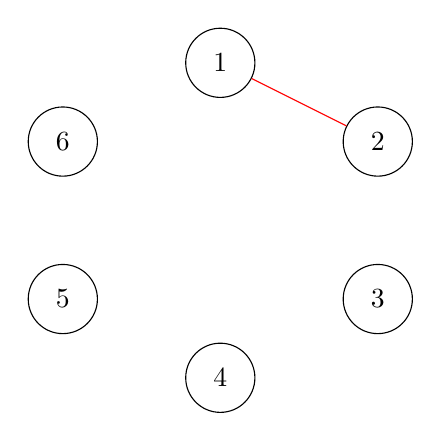
\begin{tikzpicture}
				\tikzstyle{Vertex} = [circle, draw, minimum size=25, inner sep=0pt]	
				\node (1) at (2,3) [Vertex, fill=white] {1};
				\node (2) at (4,2) [Vertex, fill=white] {2};
				\node (3) at (4,0) [Vertex, fill=white] {3};
				\node (4) at (2,-1) [Vertex, fill=white] {4};
				\node (5) at (0,0) [Vertex, fill=white] {5};
				\node (6) at (0,2) [Vertex, fill=white] {6};
				\draw[red] [-] (1) to (2);
			\end{tikzpicture}
		\end{center}
	
		\begin{align*}
			P &= (\cancel{1},{\color{red}\cancel{1}},1,1)\\
			L &= (1,\cancel{2},{\color{red}\cancel{3}},4,5,6)
		\end{align*}
		\begin{center}
			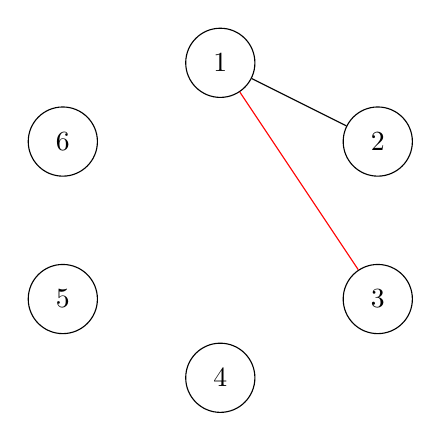
\begin{tikzpicture}
				\tikzstyle{Vertex} = [circle, draw, minimum size=25, inner sep=0pt]	
				\node (1) at (2,3) [Vertex, fill=white] {1};
				\node (2) at (4,2) [Vertex, fill=white] {2};
				\node (3) at (4,0) [Vertex, fill=white] {3};
				\node (4) at (2,-1) [Vertex, fill=white] {4};
				\node (5) at (0,0) [Vertex, fill=white] {5};
				\node (6) at (0,2) [Vertex, fill=white] {6};
				\draw [-] (1) to (2);
				\draw[red] [-] (1) to (3);
			\end{tikzpicture}
		\end{center}
	
		\begin{align*}
			P &= (\cancel{1},\cancel{1},{\color{red}\cancel{1}},1)\\
			L &= (1,\cancel{2},\cancel{3},{\color{red}\cancel{4}},5,6)
		\end{align*}
		\begin{center}
			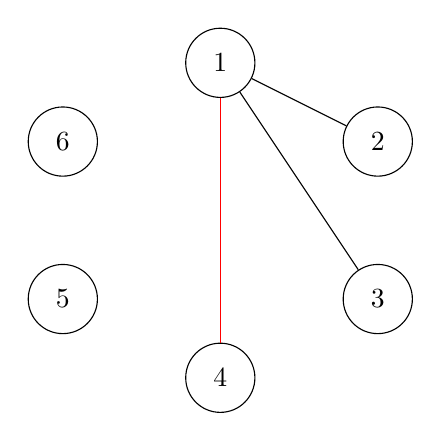
\begin{tikzpicture}
				\tikzstyle{Vertex} = [circle, draw, minimum size=25, inner sep=0pt]	
				\node (1) at (2,3) [Vertex, fill=white] {1};
				\node (2) at (4,2) [Vertex, fill=white] {2};
				\node (3) at (4,0) [Vertex, fill=white] {3};
				\node (4) at (2,-1) [Vertex, fill=white] {4};
				\node (5) at (0,0) [Vertex, fill=white] {5};
				\node (6) at (0,2) [Vertex, fill=white] {6};
				\draw [-] (1) to (2);
				\draw [-] (1) to (3);
				\draw[red] [-] (1) to (4);
			\end{tikzpicture}
		\end{center}
	
		\begin{align*}
			P &= (\cancel{1},\cancel{1},\cancel{1},{\color{red}\cancel{1}})\\
			L &= (1,\cancel{2},\cancel{3},\cancel{4},{\color{red}\cancel{5}},6)
		\end{align*}
		\begin{center}
			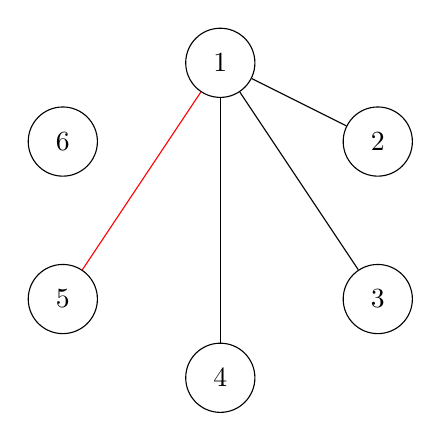
\begin{tikzpicture}
				\tikzstyle{Vertex} = [circle, draw, minimum size=25, inner sep=0pt]	
				\node (1) at (2,3) [Vertex, fill=white] {1};
				\node (2) at (4,2) [Vertex, fill=white] {2};
				\node (3) at (4,0) [Vertex, fill=white] {3};
				\node (4) at (2,-1) [Vertex, fill=white] {4};
				\node (5) at (0,0) [Vertex, fill=white] {5};
				\node (6) at (0,2) [Vertex, fill=white] {6};
				\draw [-] (1) to (2);
				\draw [-] (1) to (3);
				\draw [-] (1) to (4);
				\draw[red] [-] (1) to (5);
			\end{tikzpicture}
		\end{center}
	
		\begin{align*}
			P &= (\cancel{1},\cancel{1},\cancel{1},\cancel{1})\\
			L &= ({\color{red}\cancel{1}},\cancel{2},\cancel{3},\cancel{4},\cancel{5},{\color{red}\cancel{6}})
		\end{align*}
		\begin{center}
			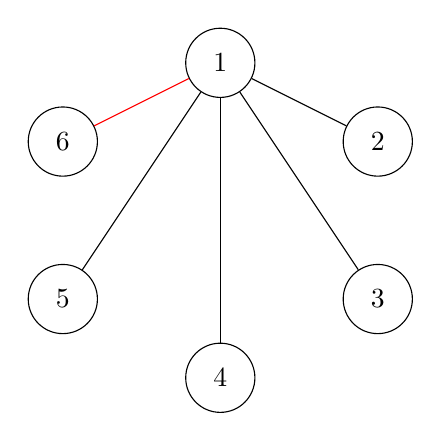
\begin{tikzpicture}
				\tikzstyle{Vertex} = [circle, draw, minimum size=25, inner sep=0pt]	
				\node (1) at (2,3) [Vertex, fill=white] {1};
				\node (2) at (4,2) [Vertex, fill=white] {2};
				\node (3) at (4,0) [Vertex, fill=white] {3};
				\node (4) at (2,-1) [Vertex, fill=white] {4};
				\node (5) at (0,0) [Vertex, fill=white] {5};
				\node (6) at (0,2) [Vertex, fill=white] {6};
				\draw [-] (1) to (2);
				\draw [-] (1) to (3);
				\draw [-] (1) to (4);
				\draw [-] (1) to (5);
				\draw[red] [-] (1) to (6);
			\end{tikzpicture}
		\end{center}
		
		Draw the second tree. Let $P = (1,1,4,4)$(You can make another code). Then we have 6 nodes. Let $L = (1,2,3,4,5,6)$.
		\begin{align*}
			P &= ({\color{red}\cancel{1}},1,4,4)\\
			L &= (1,{\color{red}\cancel{2}},3,4,5,6)
		\end{align*}
		\begin{center}
			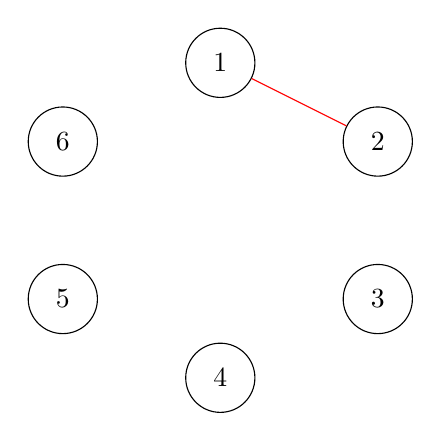
\begin{tikzpicture}
				\tikzstyle{Vertex} = [circle, draw, minimum size=25, inner sep=0pt]	
				\node (1) at (2,3) [Vertex, fill=white] {1};
				\node (2) at (4,2) [Vertex, fill=white] {2};
				\node (3) at (4,0) [Vertex, fill=white] {3};
				\node (4) at (2,-1) [Vertex, fill=white] {4};
				\node (5) at (0,0) [Vertex, fill=white] {5};
				\node (6) at (0,2) [Vertex, fill=white] {6};
				\draw[red] [-] (1) to (2);
			\end{tikzpicture}
		\end{center}
		
		\begin{align*}
			P &= (\cancel{1},{\color{red}\cancel{1}},4,4)\\
			L &= (1,\cancel{2},{\color{red}\cancel{3}},4,5,6)
		\end{align*}
		\begin{center}
			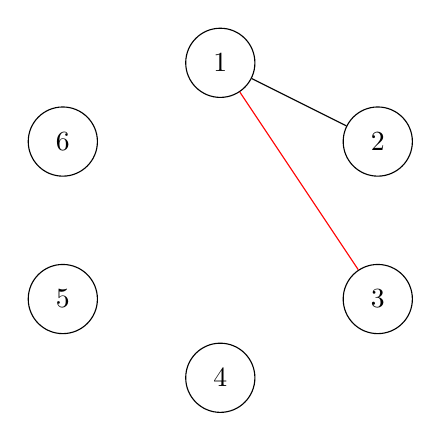
\begin{tikzpicture}
				\tikzstyle{Vertex} = [circle, draw, minimum size=25, inner sep=0pt]	
				\node (1) at (2,3) [Vertex, fill=white] {1};
				\node (2) at (4,2) [Vertex, fill=white] {2};
				\node (3) at (4,0) [Vertex, fill=white] {3};
				\node (4) at (2,-1) [Vertex, fill=white] {4};
				\node (5) at (0,0) [Vertex, fill=white] {5};
				\node (6) at (0,2) [Vertex, fill=white] {6};
				\draw [-] (1) to (2);
				\draw[red] [-] (1) to (3);
			\end{tikzpicture}
		\end{center}
		
		\begin{align*}
			P &= (\cancel{1},\cancel{1},{\color{red}\cancel{4}},4)\\
			L &= ({\color{red}\cancel{1}},\cancel{2},\cancel{3},4,5,6)
		\end{align*}
		\begin{center}
			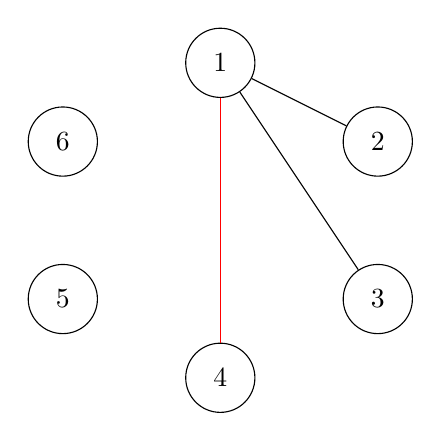
\begin{tikzpicture}
				\tikzstyle{Vertex} = [circle, draw, minimum size=25, inner sep=0pt]	
				\node (1) at (2,3) [Vertex, fill=white] {1};
				\node (2) at (4,2) [Vertex, fill=white] {2};
				\node (3) at (4,0) [Vertex, fill=white] {3};
				\node (4) at (2,-1) [Vertex, fill=white] {4};
				\node (5) at (0,0) [Vertex, fill=white] {5};
				\node (6) at (0,2) [Vertex, fill=white] {6};
				\draw [-] (1) to (2);
				\draw [-] (1) to (3);
				\draw[red] [-] (1) to (4);
			\end{tikzpicture}
		\end{center}
		
		\begin{align*}
			P &= (\cancel{1},\cancel{1},\cancel{4},{\color{red}\cancel{4}})\\
			L &= (\cancel{1},\cancel{2},\cancel{3},4,{\color{red}\cancel{5}},6)
		\end{align*}
		\begin{center}
			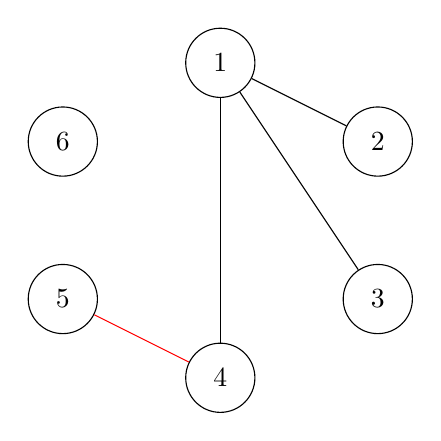
\begin{tikzpicture}
				\tikzstyle{Vertex} = [circle, draw, minimum size=25, inner sep=0pt]	
				\node (1) at (2,3) [Vertex, fill=white] {1};
				\node (2) at (4,2) [Vertex, fill=white] {2};
				\node (3) at (4,0) [Vertex, fill=white] {3};
				\node (4) at (2,-1) [Vertex, fill=white] {4};
				\node (5) at (0,0) [Vertex, fill=white] {5};
				\node (6) at (0,2) [Vertex, fill=white] {6};
				\draw [-] (1) to (2);
				\draw [-] (1) to (3);
				\draw [-] (1) to (4);
				\draw[red] [-] (4) to (5);
			\end{tikzpicture}
		\end{center}
		
		\begin{align*}
			P &= (\cancel{1},\cancel{1},\cancel{4},\cancel{4})\\
			L &= (\cancel{1},\cancel{2},\cancel{3},{\color{red}\cancel{4}},\cancel{5},{\color{red}\cancel{6}})
		\end{align*}
		\begin{center}
			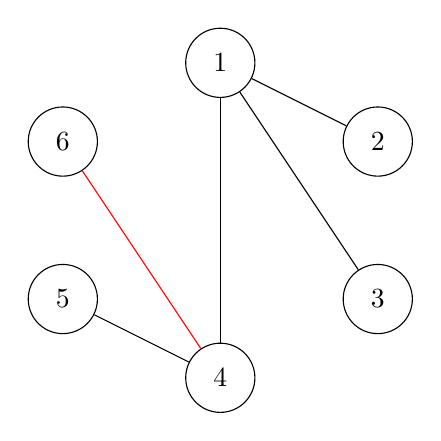
\begin{tikzpicture}
				\tikzstyle{Vertex} = [circle, draw, minimum size=25, inner sep=0pt]	
				\node (1) at (2,3) [Vertex, fill=white] {1};
				\node (2) at (4,2) [Vertex, fill=white] {2};
				\node (3) at (4,0) [Vertex, fill=white] {3};
				\node (4) at (2,-1) [Vertex, fill=white] {4};
				\node (5) at (0,0) [Vertex, fill=white] {5};
				\node (6) at (0,2) [Vertex, fill=white] {6};
				\draw [-] (1) to (2);
				\draw [-] (1) to (3);
				\draw [-] (1) to (4);
				\draw [-] (4) to (5);
				\draw[red] [-] (4) to (6);
			\end{tikzpicture}
		\end{center}
	\end{proof}